\documentclass[a4paper]{article}

% Set for specific document
\def\DOCTITLE{Software Rasteriser Screenshots}
\def\DOCAUTHOR{Dan Nixon (120263697)}
\def\DOCDATE{16/11/2015}

% Set document attributes
\title{\DOCTITLE}
\author{\DOCAUTHOR}
\date{\DOCDATE}

\usepackage{fullpage}
\usepackage{scrextend}
\usepackage{titlesec}
\usepackage{fancyhdr}

% Handle graphics correctly
\ifx\pdftexversion\undefined
\usepackage{graphicx}
% \usepackage[dvips]{graphicx}
\else
\usepackage[pdftex]{graphicx}
\DeclareGraphicsRule{*}{mps}{*}{}
\fi

% Setup headers and footers
\pagestyle{fancy}
\lhead{}
\chead{\DOCTITLE}
\rhead{}
\rfoot{\DOCDATE}
\cfoot{\thepage}
\lfoot{\DOCAUTHOR}

% New page for each section
\newcommand{\sectionbreak}{\clearpage}

% Set header and footer sizes
\renewcommand{\headrulewidth}{0.4pt}
\renewcommand{\footrulewidth}{0.4pt}
\setlength{\headheight}{15.2pt}
\setlength{\headsep}{15.2pt}

\begin{document}

% \begin{figure}[h!]
  % \centering
  % 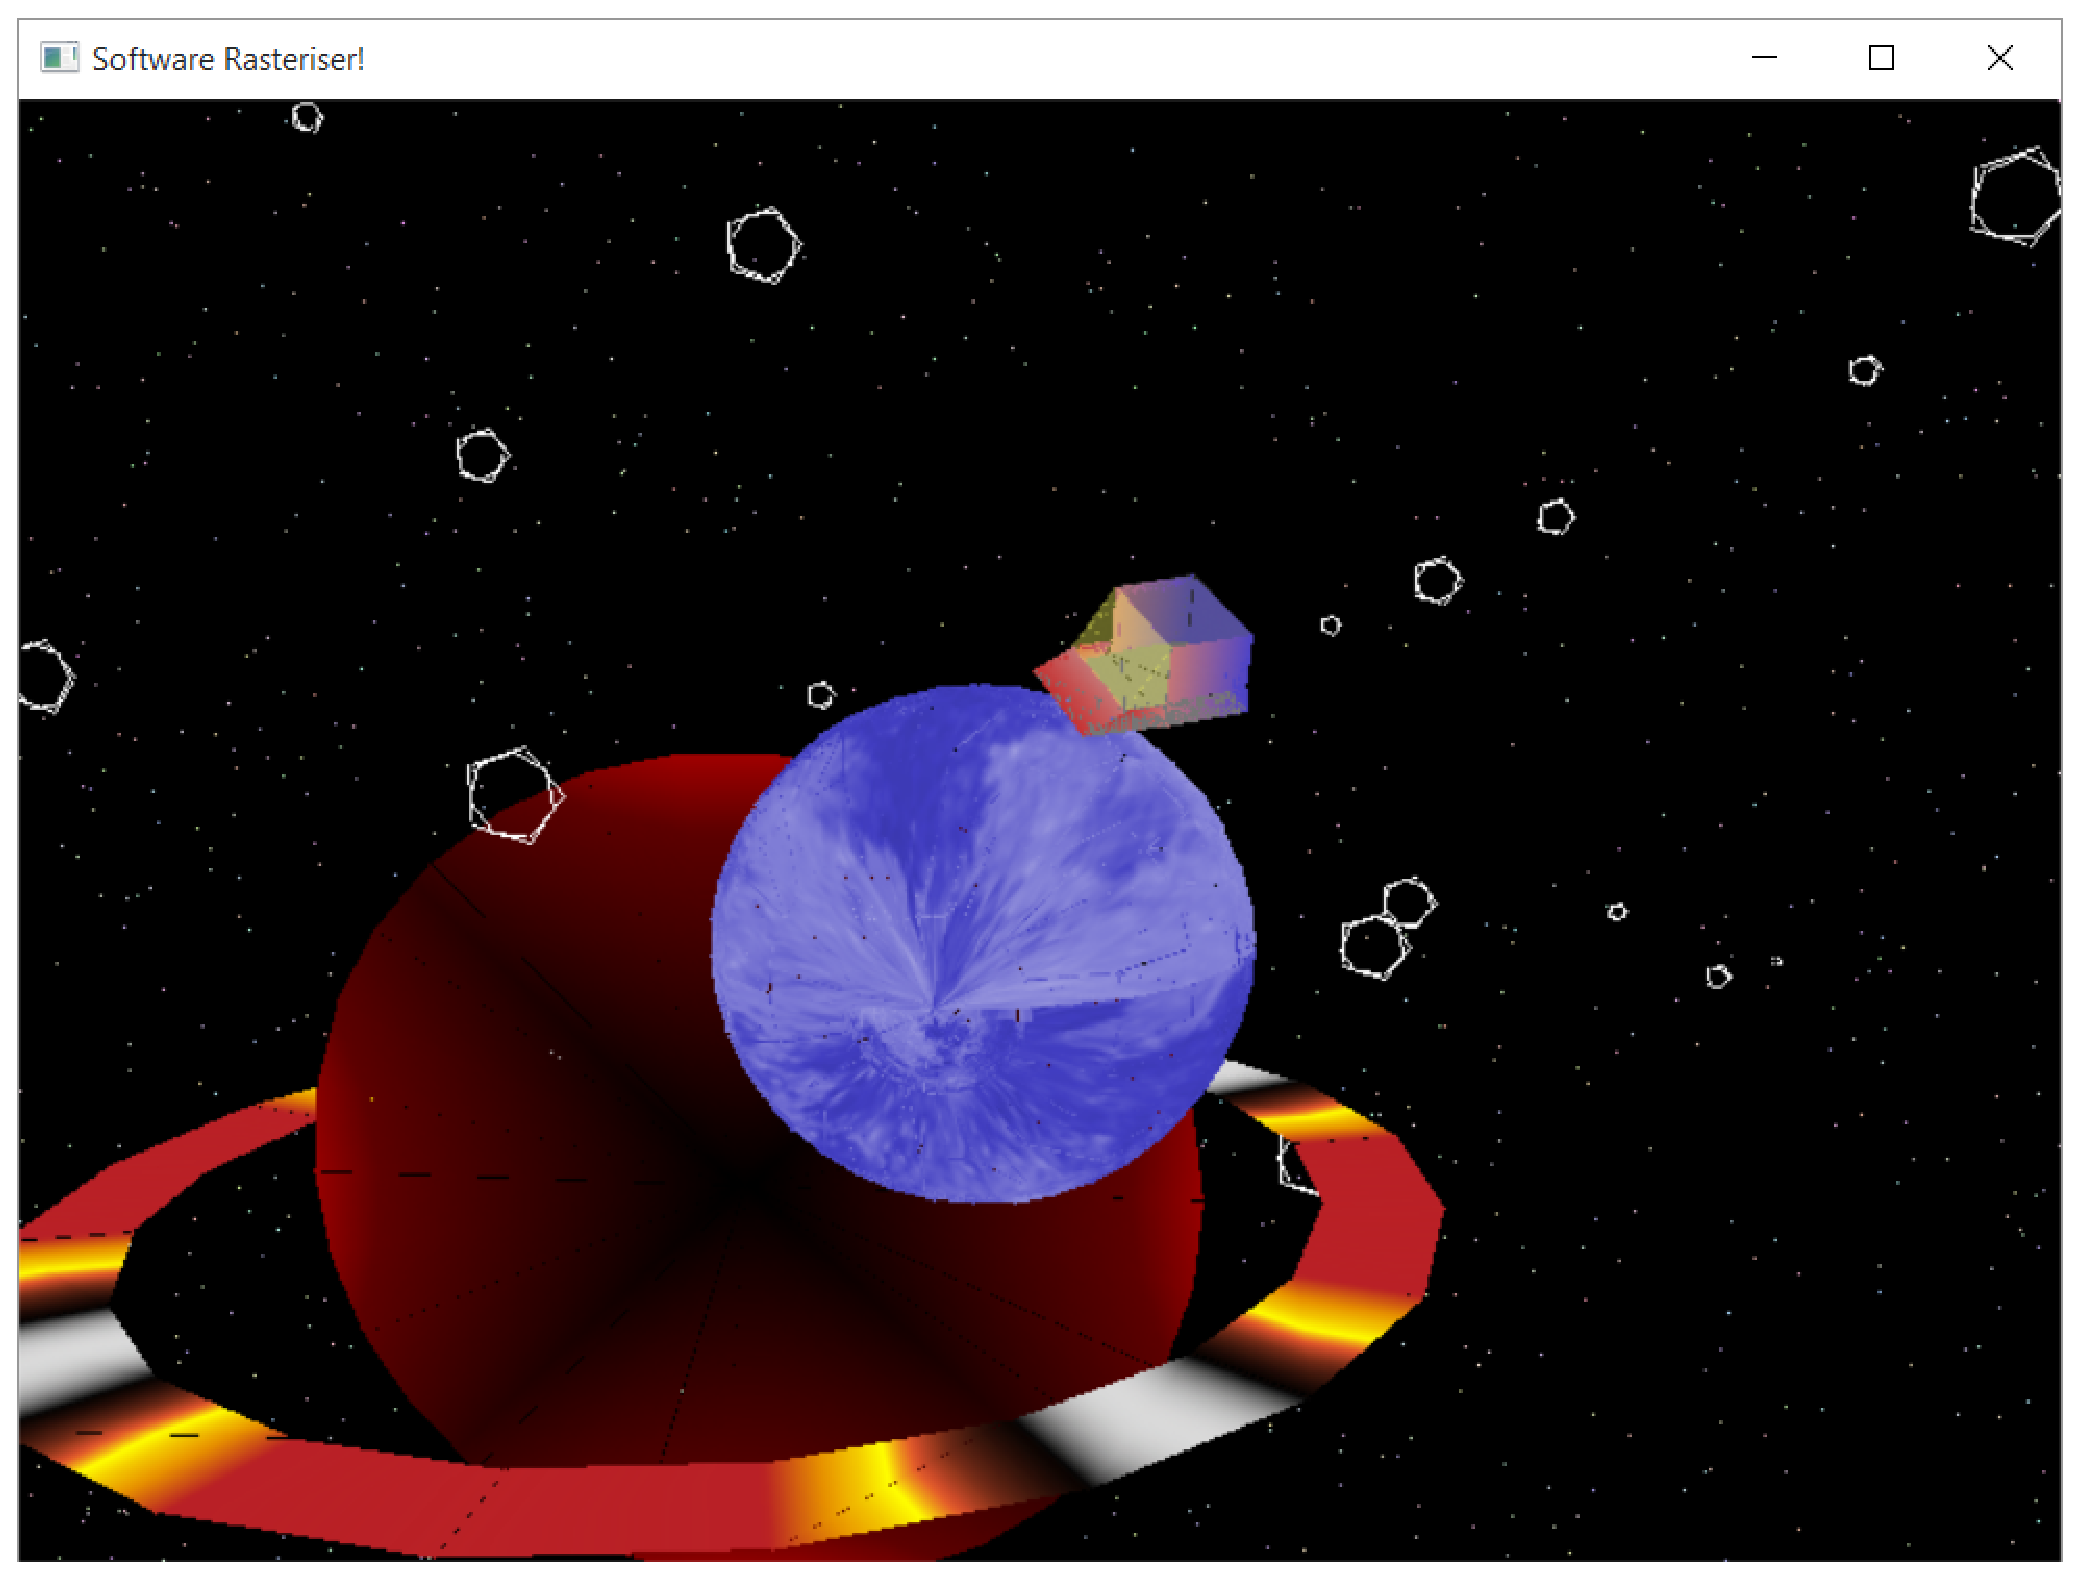
\includegraphics[width=0.85\textwidth]{graphics/screen_1.eps}
  % \caption{Spaceship, moon and planet}
  % \label{fig:screen_1}
% \end{figure}

\begin{figure}[h!]
  \centering
  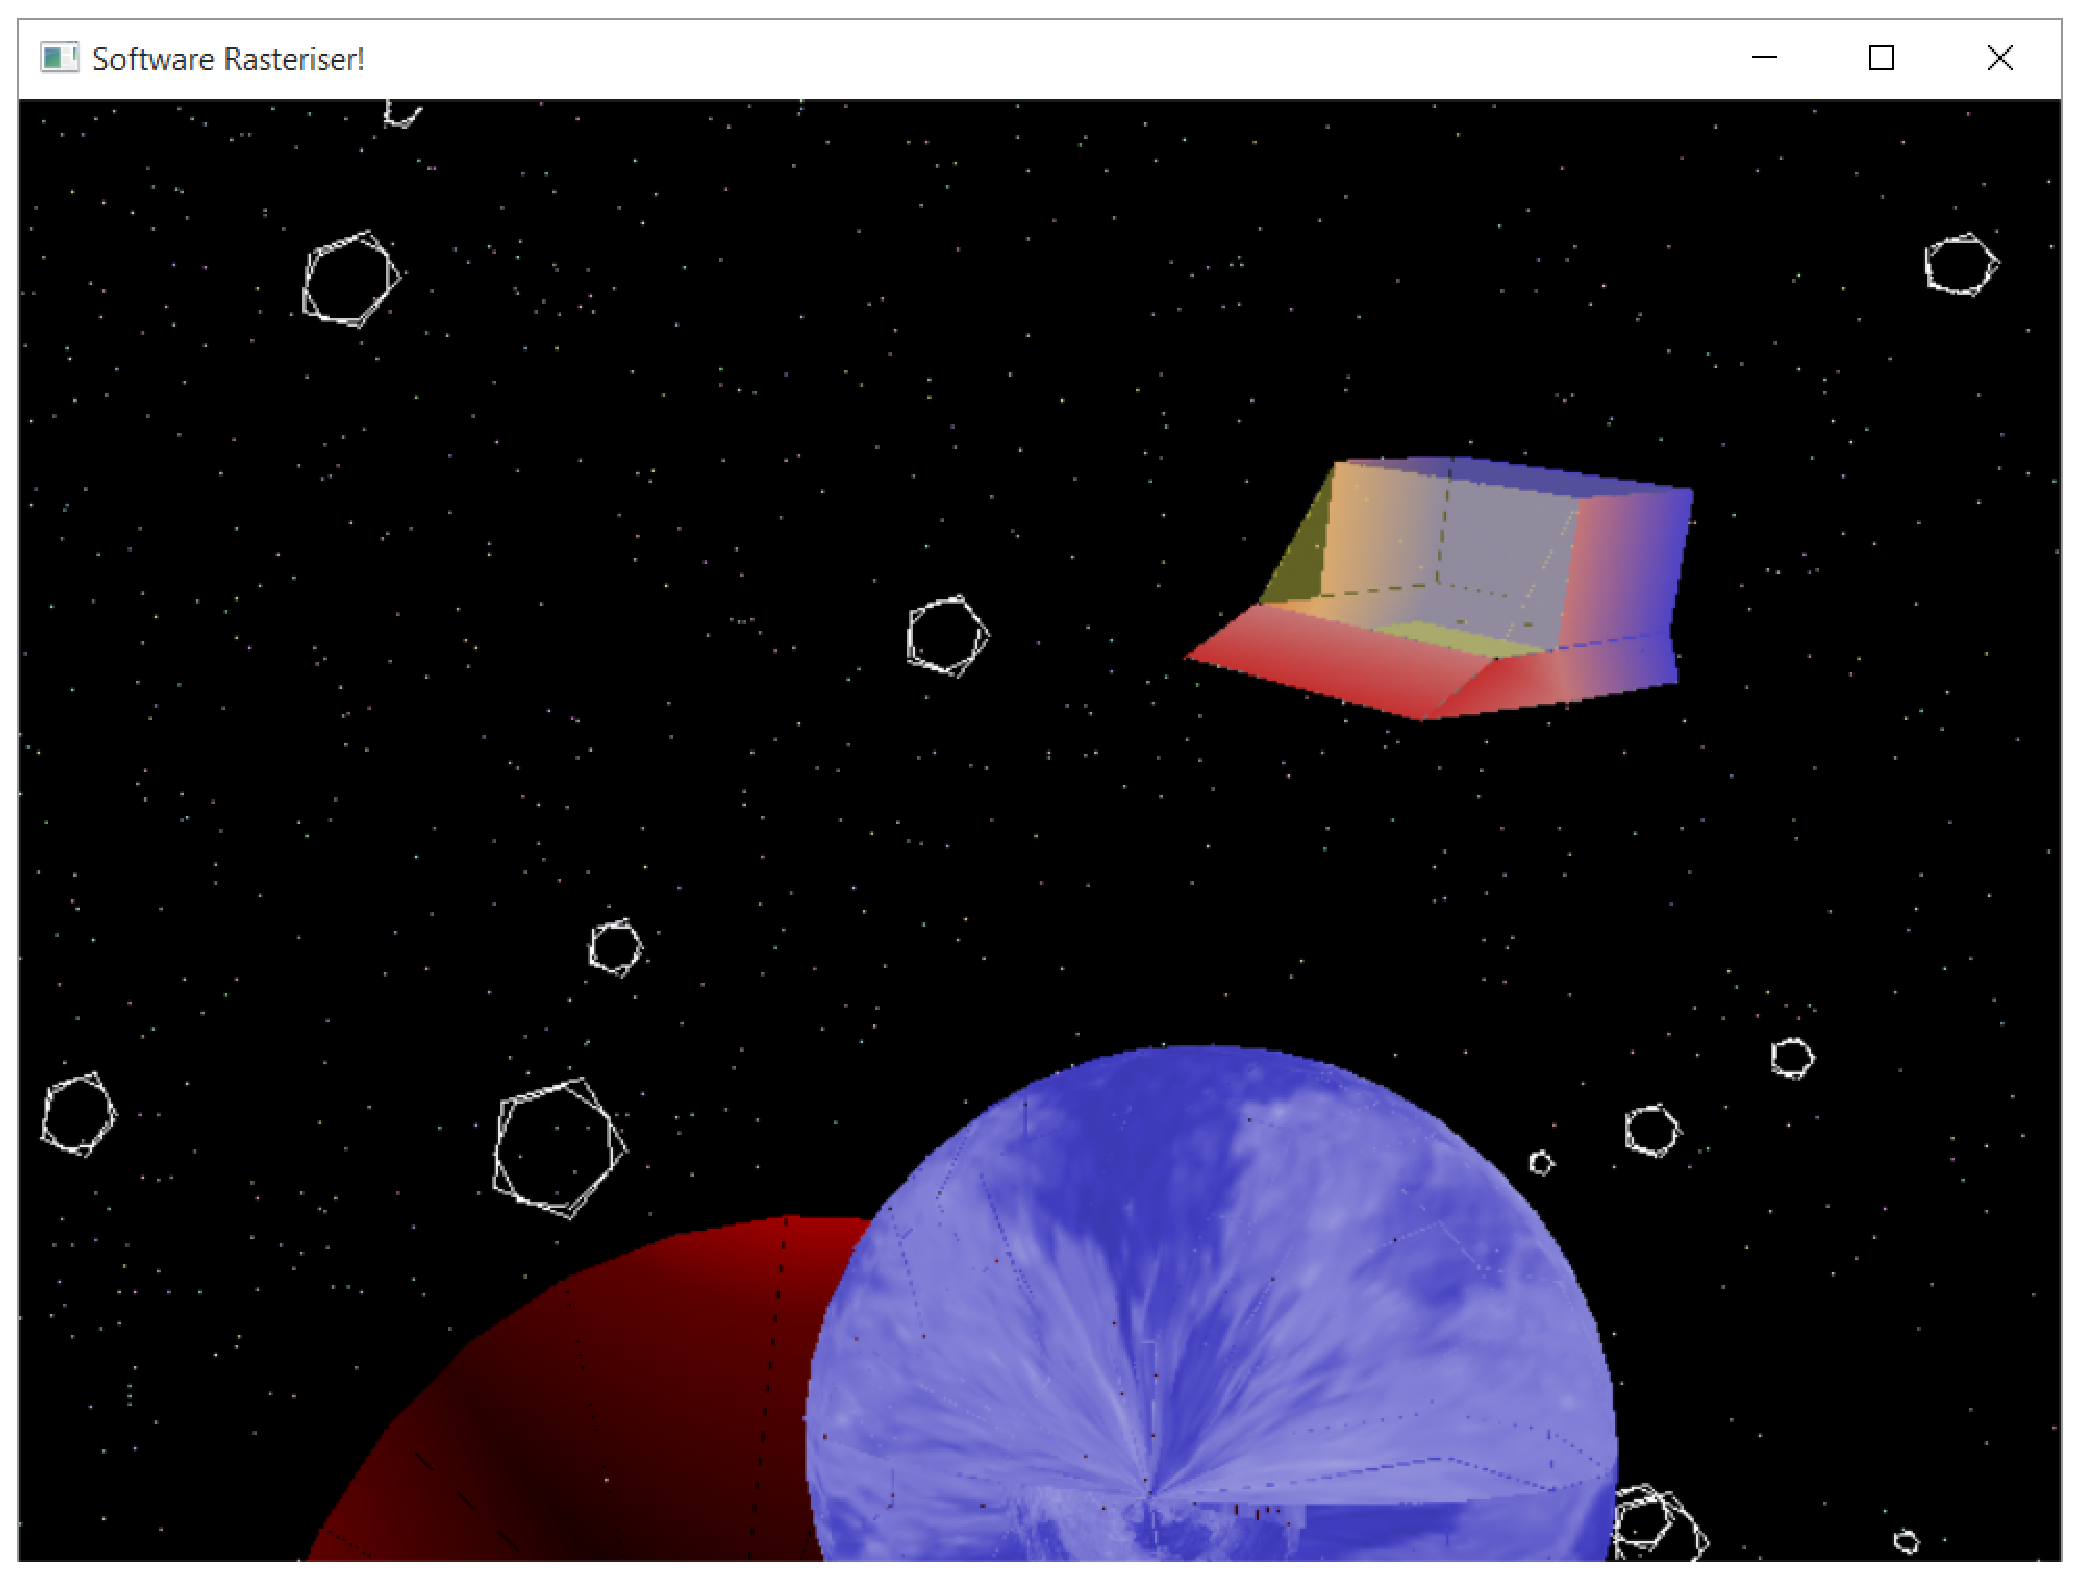
\includegraphics[width=0.85\textwidth]{graphics/screen_2.eps}
  \caption{Spaceship}
  \label{fig:screen_2}
\end{figure}

\begin{figure}[h!]
  \centering
  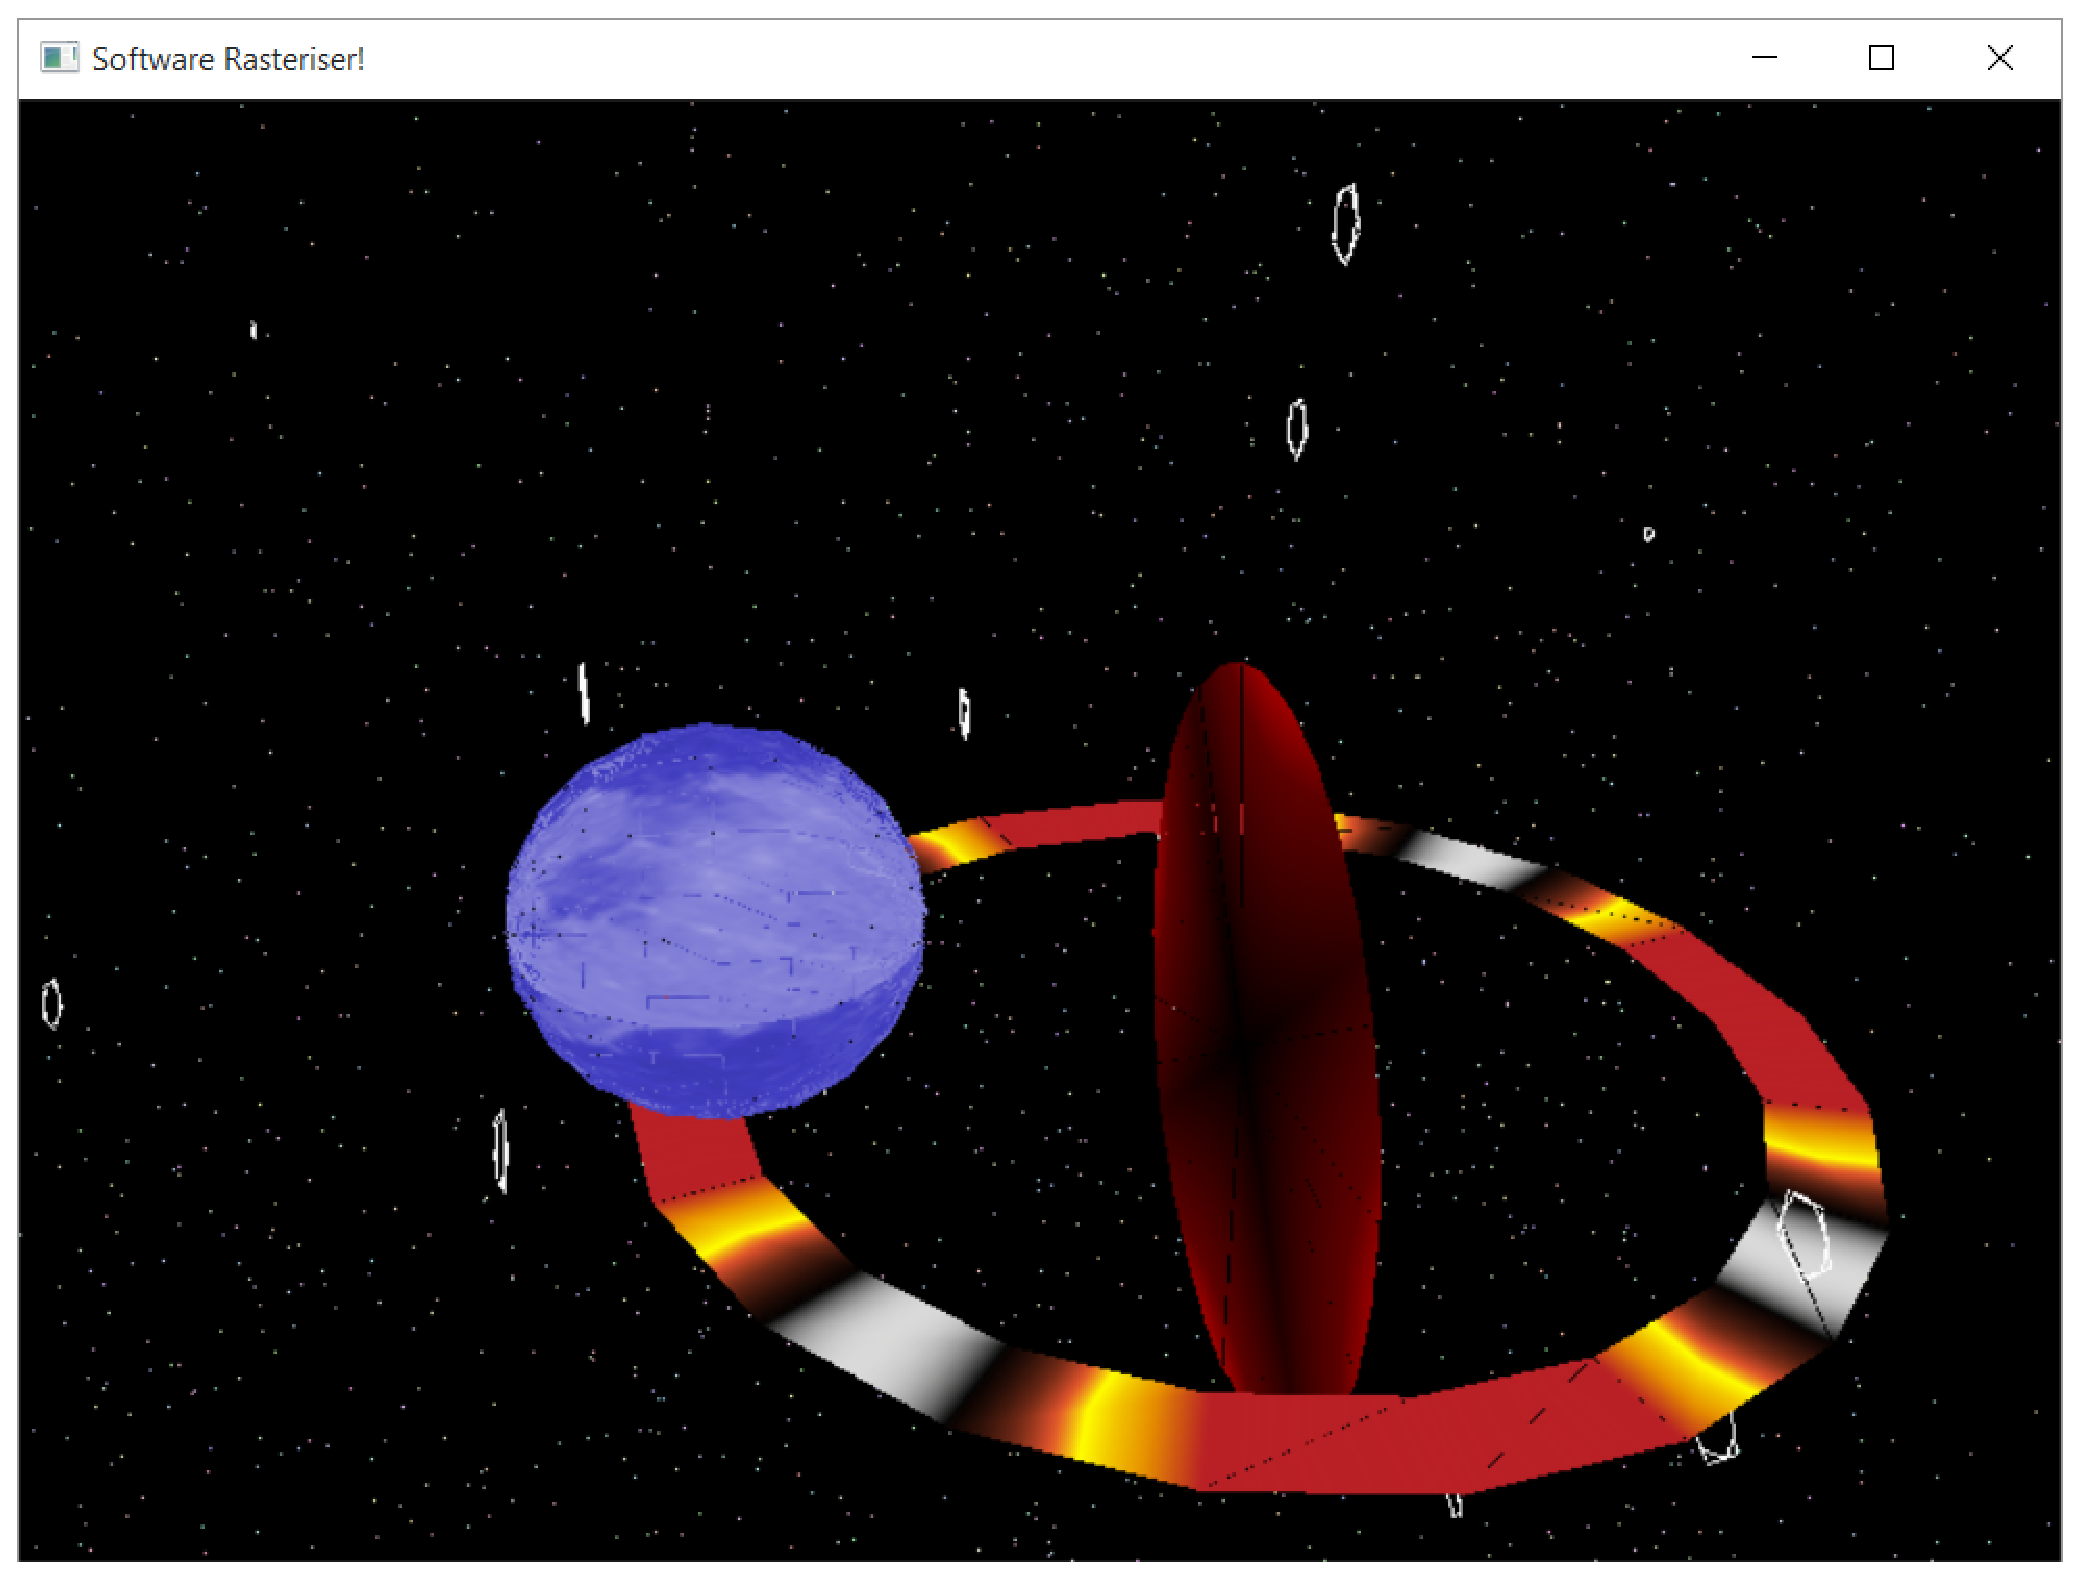
\includegraphics[width=0.85\textwidth]{graphics/screen_3.eps}
  \caption{Side view of 3D moon and 2D planet}
  \label{fig:screen_3}
\end{figure}

\begin{figure}[h!]
  \centering
  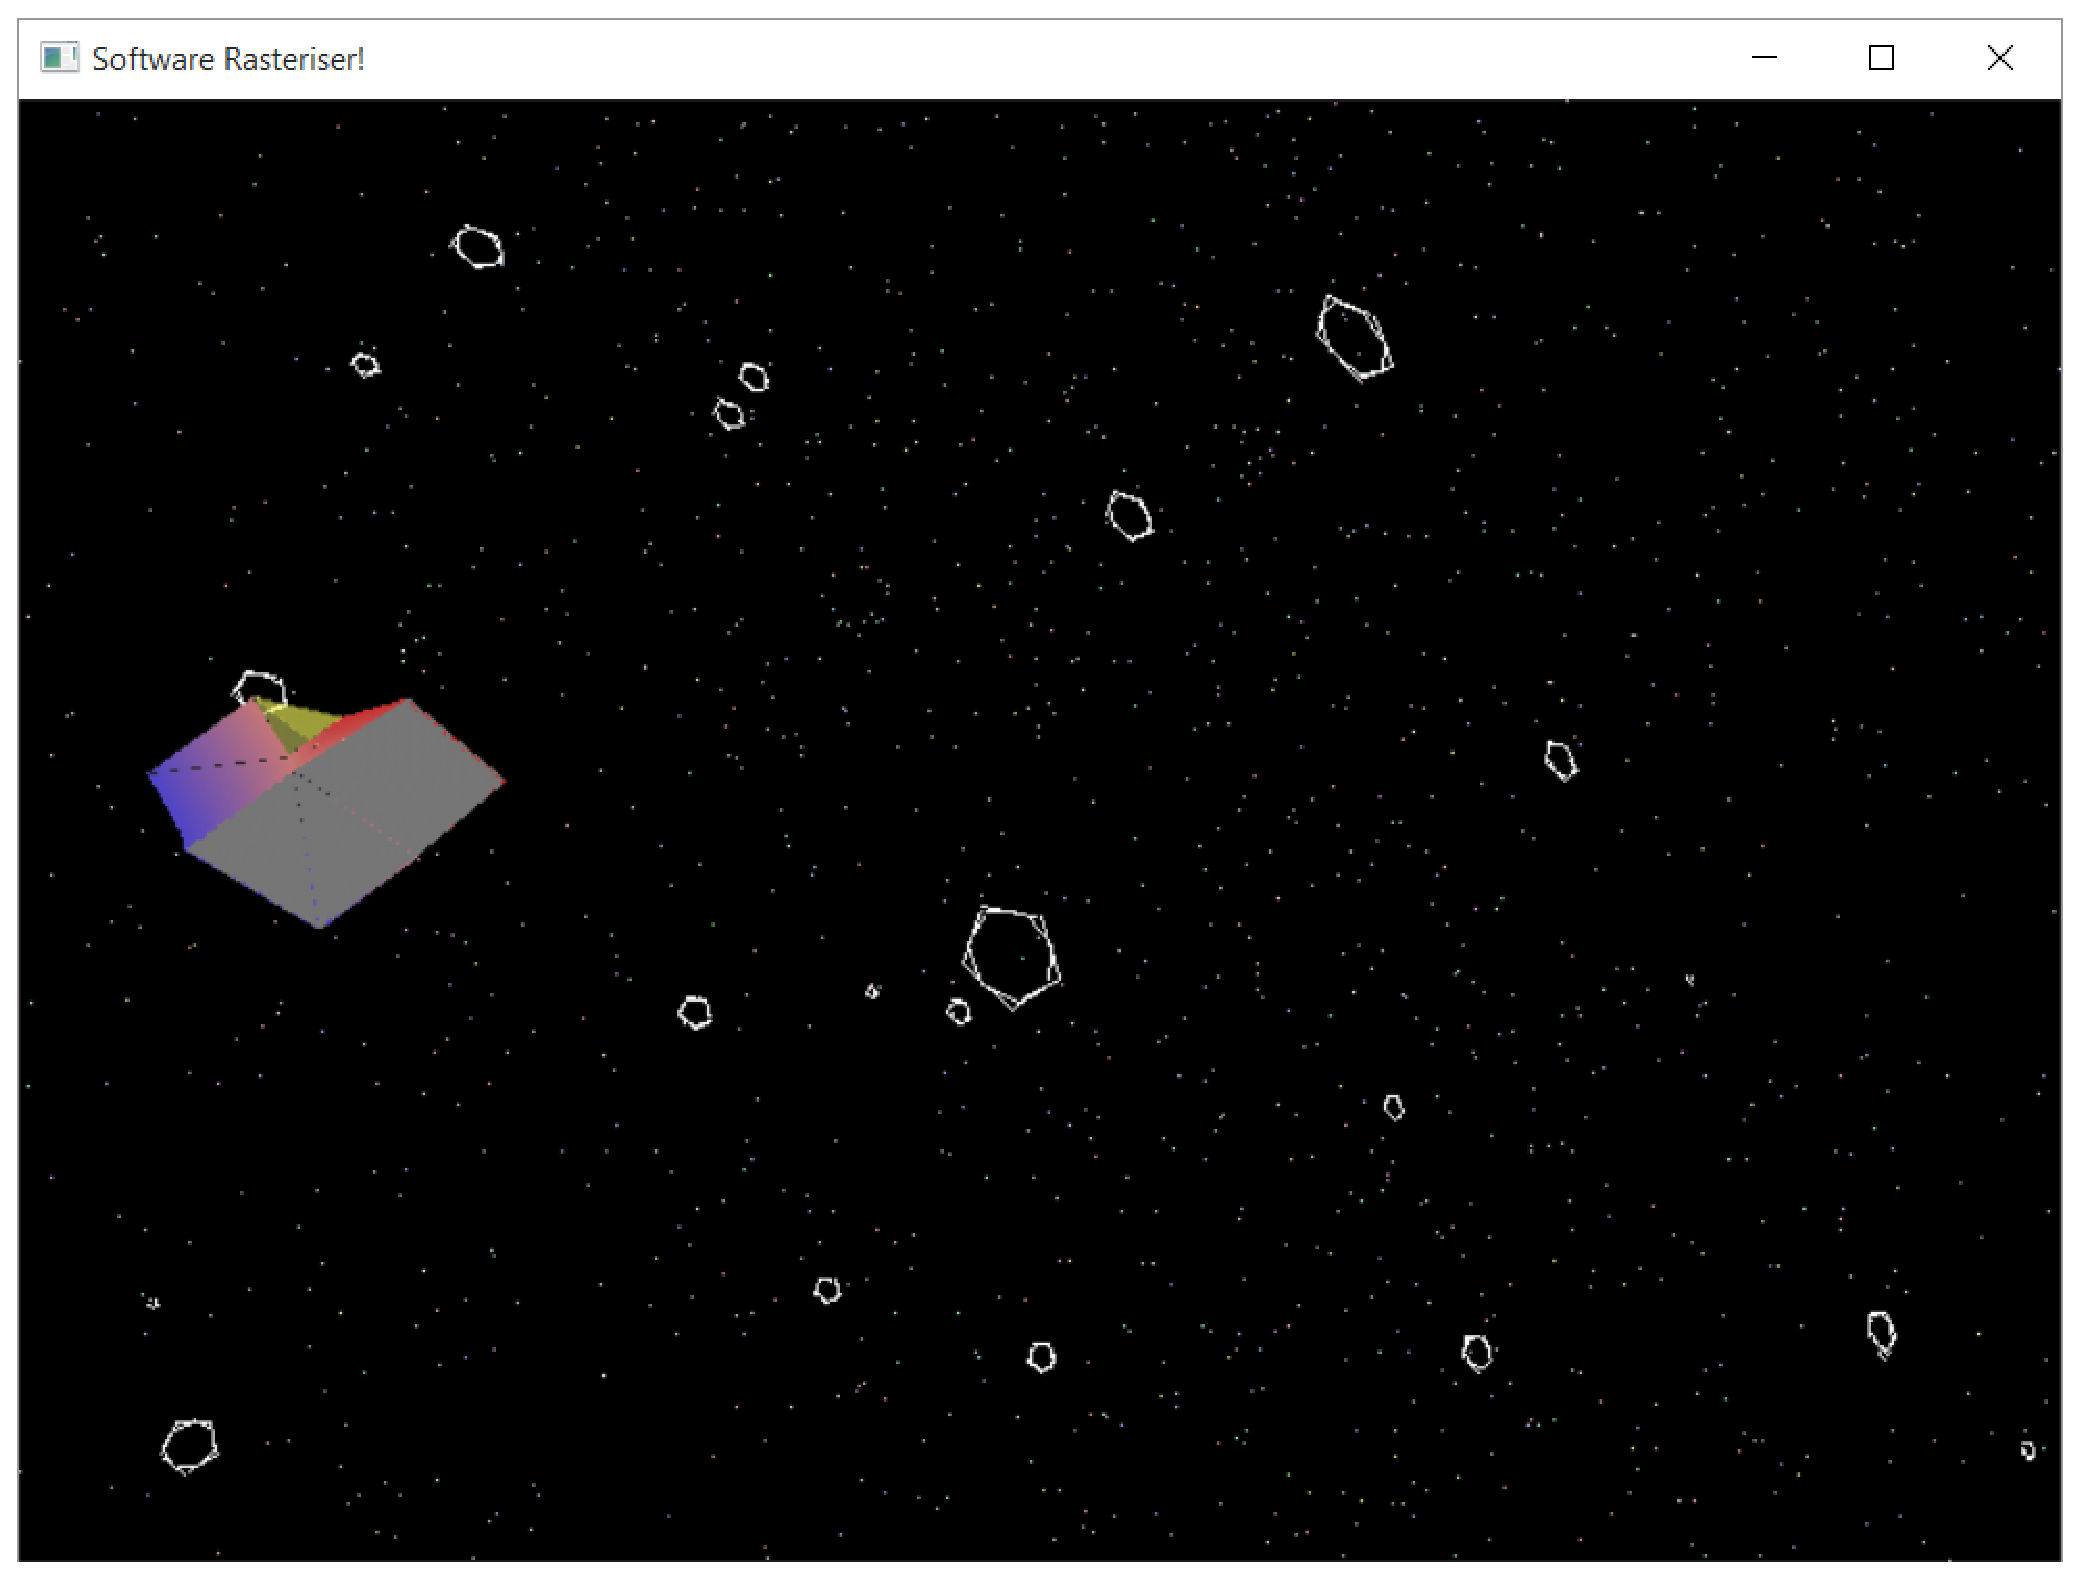
\includegraphics[width=0.85\textwidth]{graphics/screen_4.eps}
  \caption{2D asteroids and star field}
  \label{fig:screen_4}
\end{figure}

\begin{figure}[h!]
  \centering
  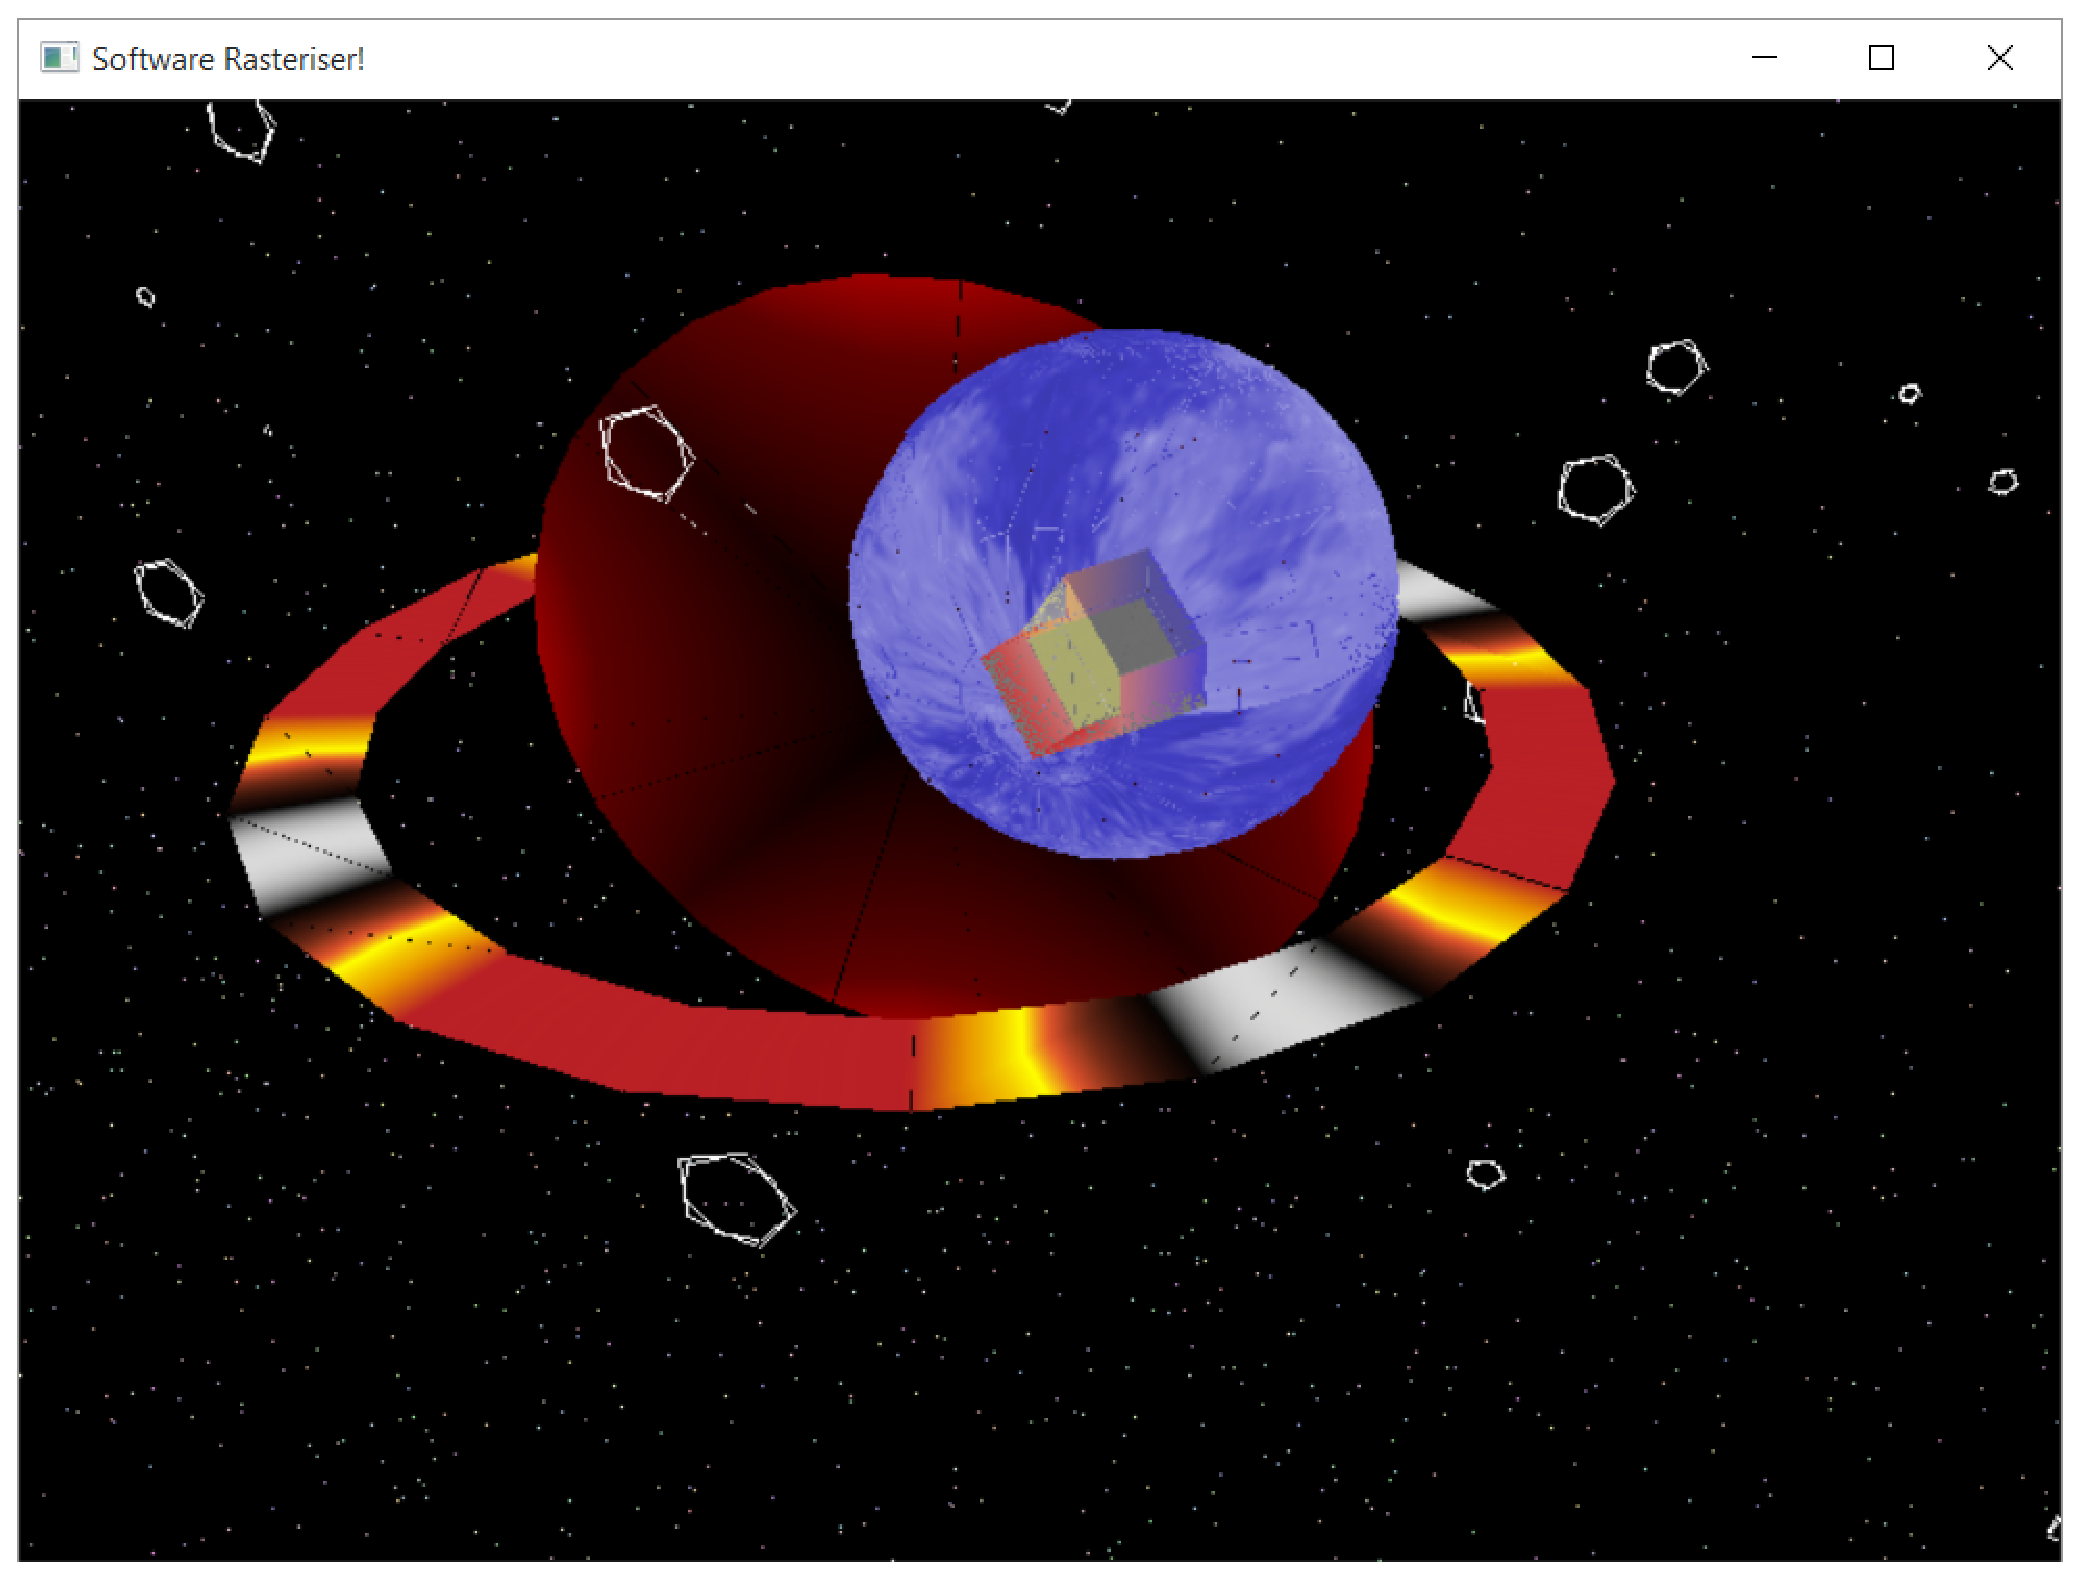
\includegraphics[width=0.85\textwidth]{graphics/screen_5.eps}
  \caption{Spaceship, moon and planet}
  \label{fig:screen_5}
\end{figure}

\end{document}
